% Use a modified ACM conference proceedings template
\documentclass[sigconf]{acmart}
% Disable some elements from ACM template
\setcopyright{none}
\settopmatter{printacmref=false,printfolios=false}

\usepackage{booktabs} % For formal tables
\usepackage[ruled,vlined]{algorithm2e}
\usepackage{amsmath} % for writing algorithms
\usepackage{cleveref}

% OWN COMMANDS
\newcommand{\todo}[1]{{\color{red}{#1}}}

% VARIABLES
\usepackage{xspace} % allows \commmand instead of \command{} with correct space afterwards
\newcommand{\VNumSimulations}{20\xspace}
\newcommand{\VNumDays}{10.000\xspace}
\newcommand{\VNumPop}{100\xspace}
\newcommand{\VNumTrees}{140\xspace}
\newcommand{\VProbPredator}{0.003\xspace}
\newcommand{\VProbAltruistDies}{0.50\xspace}
\newcommand{\VProbKids}{0.001\xspace}


\newcommand{\cowards}{\textit{cowards}\xspace}
\newcommand{\coward}{\textit{coward}\xspace}
\newcommand{\altruist}{\textit{altruist}\xspace}
\newcommand{\altruists}{\textit{altruists}\xspace}
\newcommand{\suckers}{\textit{suckers}\xspace}
\newcommand{\sucker}{\textit{sucker}\xspace}
\newcommand{\impostors}{\textit{impostors}\xspace}
\newcommand{\impostor}{\textit{impostor}\xspace}
\newcommand{\greenbeards}{\textit{greenbeards}\xspace}
\newcommand{\greenbeard}{\textit{greenbeard}\xspace}


\begin{document}
    \title{On Trust and Prosociality}

    \author{Fatjon Zogaj}\affiliation{}
    \email{fzogaj@student.ethz.ch}

    \author{Rafael Sterzinger}\affiliation{}
    \email{rsterzinger@student.ethz.ch}

    \begin{abstract}
        \todo{Briefly summarize your report here. This should include a description of the task you are solving, a summary of how you approach the task (i.e. your method), as well as a preview of the central result. The abstract should be short, i.e. 4-5 sentences. The rest of this template outlines a rough structure how you \emph{can} organize your report. It mentions all the components we would typically expect. It is a good idea to adhere these guidelines, but they are not binding, i.e., you are free to re-organize your report as you see fit.}
    \end{abstract}

    \maketitle


    \section{Introduction}\label{sec:introduction}
    %\todo{In this section, introduce the task in a bit more detail. In the first paragraph, try to answer why the task is of interest at all and what makes it challenging. You may also discuss some related work here. For example, you can summarize how other researchers have addressed the problem and what might be the disadvantages of these works.}


    The evolution of cooperation is a question which has been bothering humanity for a long time.
    Not only is it open for debate in the fields of anthropology, sociology, and economy but also evolutionary biologist have tried to answer this question on multiple occasions \cite{gardner_theory_2009}.
    Hence, in 2005, at the 125th anniversary issue of the American Association for the Advancement of Science (AAAS), they declared the question "How Did Cooperative Behavior Evolve?" to be one of the top 25 unsolved puzzles science is facing over the next quarter century \cite{aaas_125th_2005}.

    Already in the year \citeyear{darwin_origin_1859}, \citeauthor{darwin_origin_1859}'s natural selection theory tried to explain the underlying mechanisms of a growing population.
    More helpful characteristics that lead to better reproduction will keep on spreading throughout the population \cite{darwin_origin_1859}.
    This gives off the impression that certain traits will develop in order to optimize an individual's reproducibility (fitness). \citeauthor{fisherGeneticalTheoryNatural1930} builds upon this by introducing the notion of gene frequencies.
    Genes leading to higher individual fitness thus will increase in frequency and lead to a general increase in mean fitness \cite{fisherGeneticalTheoryNatural1930}.


    %\todo{In the second half of the introduction, describe your method. This should be more detailed than in the abstract. You can talk about how your method relates to existing work (e.g. it is a combination or extension of existing methods, what other papers were you inspired by, etc.). You should also state the central result here, and the key insight that made it possible to achieve this result.}

    \todo{relate this to related work/experiments}

    In this work, we conduct a variety of experiments to analyze how different levels of cooperation and environment settings affect a population and the development of the respective types/tribes within.
    For this we run \VNumSimulations, each spanning \VNumDays and visualize the average results of those runs.
    The general environment looks as follows.
    Based on a starting population of \VNumPop, these starting agents compete for \VNumTrees possible jobs to win money every day.
    One of these jobs enables up to 2 agents to live on as they can be split, without changing any outcome.
    To simplify the case, we say that if an agent is not able to win any of the $2 \times \VNumTrees$ job option, he goes bankrupt and dies out.
    On top of that, not every one of the jobs is a guaranteed win.
    With a certain probability \VProbPredator an option is considered to be hard and if only one agent has taken on that job, he dies out.
    If there are two agents taking on a hard job, in the general case only one of the two is able to win while the other dies out (randomly chosen).
    This can be thought of as the company offering a hard job only being content with one of the agents and not paying the other.


    \begin{enumerate}
        \item In our first experiment we create a stable environment so that the population without any kind of certain type/tribe logic would stay roughly the same.

        \item Next we introduce altruistic thinking.
        As such, an altruist helps out the other person they are sharing a hard job with.
        By doing so, the other person is able to live on while the helping altruist now has the burden of doing both job options.
        We say that with a certain probability \VProbAltruistDies, the altruist fails and ends up sacrificing themself for the other.
        In the case that they end up succeeding however, it leads to a net-positive regarding the population size as both agents sharing the hard job are then able to live on.

        \item Building upon the previous experiment we introduce a fairer notion, where \greenbeards only help out other \greenbeards.

        \item A final experiment introduces further types next to the altruist.
        The final types are \cowards (never help with hard jobs), \suckers (always help with hard jobs), \impostors (look like altruists, but never help) and  \greenbeards (only help other altruists, aka \suckers, \impostors and \greenbeards).

    \end{enumerate}

    We analyze these cases with a variety of different parameters which are explained in further detail in \Cref{sec:method} and \Cref{sec:results}.
    % explain in further detail in Method part

    \todo{Mention central results and key insight briefly.}


    \section{Inclusive Fitness}\label{sec:inclusive-fitness}

    Already back in the days when \citeauthor{darwin_origin_1859} developed his theory on the origin of species~\cite{darwin_origin_1859}, the idea of cooperative behaviour stood in contrast to his beliefs of natural selection and the fitness of individuals, that is the reproductive success that allows a species to dominate one another \cite{pennisi_how_2005}.
    Here, the key problem was that maximization of individual fitness does not align with the occurrence of altruistic or spiteful traits as acting cooperatively is costly and therefore would lower their own fitness level \cite{west_altruism_2010}.
    \citeauthor{darwin_origin_1859} later describes scenarios in which altruism could indirectly improve the individual fitness by cooperating among kin, i.e. supporting the transmission of underlying genes \cite{pennisi_how_2005,gardner_theory_2009}.
    This idea was later picked up by \citeauthor{hamilton_kin_1964} who has formalized \citeauthor{darwin_origin_1859}'s idea and proposed \citeauthor{hamilton_kin_1964}'s rule:

    \begin{equation}
        rb-c>0\label{eq:rb-c}
    \end{equation}


    This inequality describes when a specific trait will be favored over another by natural selection.
    Here, $c$ denotes the costs of being altruistic for the actor, $b$ encapsulates the benefit of the altruistic act for the recipient, and $r$ is a measure of the genetic relatedness between the actor and the recipient \cite{west_altruism_2010}.
    This formulation is also known as inclusive fitness which is a composition of direct fitness (\Cref{subsec:direct_fit}), i.e. the improvement of individual fitness, and indirect fitness (\Cref{subsec:indirect_fitness}), i.e. enhancing the reproductive success of other genetic related individuals.
    \Cref{fig:hamilton} summarizes this composition graphically.

    Indirect fitness can most easily be observed through interactions with others of the same kin.
    Kin here refers to somebody else sharing the common trait of genes that are inherited from one common ancestor.
    Indirect fitness is often also called \textit{Kin Selection} \cite{west_altruism_2010}.

    For the introduction of the different subcategories of direct and indirect fitness, we will borrow definitions from the more recent work by \citeauthor{west_altruism_2010} \cite{west_altruism_2010} instead of the work by \citeauthor{gardner_theory_2009} \cite{gardner_theory_2009}.

    \begin{figure}
        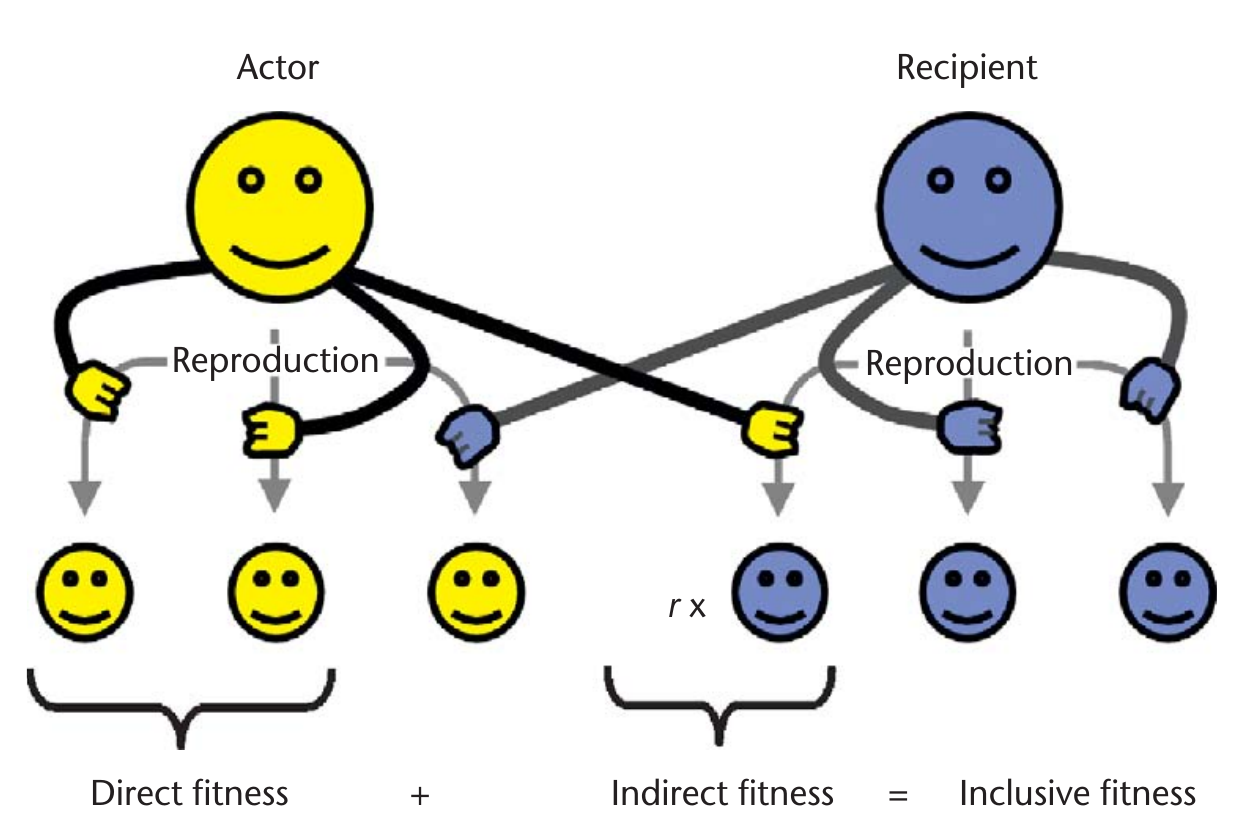
\includegraphics[width=\columnwidth]{figures/hamiltons_rule}
        \caption{\citeauthor{hamilton_kin_1964}'s rule describes inclusive fitness which consists of direct fitness $-c$ and indirect fitness $rb$. With this rule, four basic types of social behaviour can be derived \cite{gardner_theory_2009}.}
        \label{fig:hamilton}
    \end{figure}

    \subsection{Direct Fitness}\label{subsec:direct_fit}

    \subsubsection{Altruism}
    One can differentiate between two different kinds of Altruism.   %source? me lol
    The first refers to the more commonly known general case of selflessness where one helps everyone, regardless of how related they are.
    This is the case which we are analyzing in our earlier experiments, where \altruists help other \altruists and \cowards.
    The other notion of altruism refers to within-kin altruism where one only collaborates with related members of the population (visualized in \Cref{fig:mechanisms} A).
    In our later experiments we also look at this other case by introducing the notion of \greenbeards which only help other beard-kins out.

    \subsubsection{Reciprocity}\label{reciprocity}
    Compared to regular altruism, Reciprocity cannot be considered truly altruistic, as the underlying mutual benefit is based on reciprocal cooperation and not selflessness~\cite{triversEvolutionReciprocalAltruism1971}.
    In the case where agents help others that have helped them before, cooperation leads to a direct fitness increase.
    This holds only if the short term cost $c$ is smaller than the long term benefit $b$.

    \subsection{Indirect Fitness}\label{subsec:indirect_fitness}

    \subsubsection{Spite}
    As part of inclusive fitness, the roots behind the theory of altruism can be found.
    On top of that we find a similar mechanism to altruism, that differs in its manifestation.
    Spiteful behaviour can be thought of as acts that harm the recipient (and potentially the actor).
    This way, while the harmed recipient may suffer from reduced fitness, one is able to indirectly cause an increase in fitness for other participants, by removing the recipient from the pool of competition~\cite{hamiltonSelfishSpitefulBehaviour1970}.

    Looking at \Cref{eq:rb-c} we consider the case where the relatedness factor $r$ can be negative.
    A negative value could stand for the fact that the recipient is further from the actor than the average population in relatedness.
    As such, even with a positive $c$ value (actor is harmed) and a negative $b$ value (recipient is harmed), the equation can be fulfilled.
    This is e.g. the case where other participant are more closely related benefit from less competition and the less related recipient gets harmed.
    Looking at \Cref{fig:mechanisms} this is visualized in Quadrant C and can be thought of as altruism towards closer kin~\cite{west_altruism_2010}.

    From the lens of our experiments the sort of \greenbeards we analyze, end up possessing spiteful traits by helping out their own kin (direct altruism), and letting the others die out (direct spite, indirect altruism).
    % summarized up until first paragraph of page 3, still a lot more that can be added

    \subsubsection{Green Beard}
    Compared to the previously mentioned cases of altruism (help out everyone or help out own kin) another form of altruism can be noted.
    According to \citeauthor{hamiltonInnateSocialAptitudes1975} for there to be indirect fitness benefits the occurence of the same genetic strain plays a role and not the kinship itself~\cite{hamiltonInnateSocialAptitudes1975} (\Cref{fig:mechanisms}).
    A certain trait or characteristic can be used to differentiate between sharers of the same gene variation and thus used to decide on whom to help.
    Natural selection here takes place in regard to that certain gene, even with no other common DNA.
    To visualize this, one can think of a gene that is responsible for the growth of a green beard where those affected individuals end up cooperating between themselves~\cite{SelfishGeneRichard}.
    Note that this holds true even if the gene does not manifest itself visually, but leads to association between gene-sharers (e.g. a social gene; social people tend to stick with social people).

    An example of this green beard phenomenon occurring in nature was discovered by \citeauthor{keller_selfish_1998} \cite{keller_selfish_1998} where they found a spiteful green beard allele in the red imported fire ant species.
    Here, worker ants wearing a certain type of allele (bearer) are able to distinguish and lure queens of a different type (non-bearer) by odour cues and execute them resulting in fitness benefits for the worker ants.

    In real life this also opens up the possibility for \textit{falsebeards} which do seem to have inherited the same gene from the outside, but in fact do not end up cooperating as expected.
    We analyze this case in our final experiment by introducing \impostors.

    \begin{figure}
        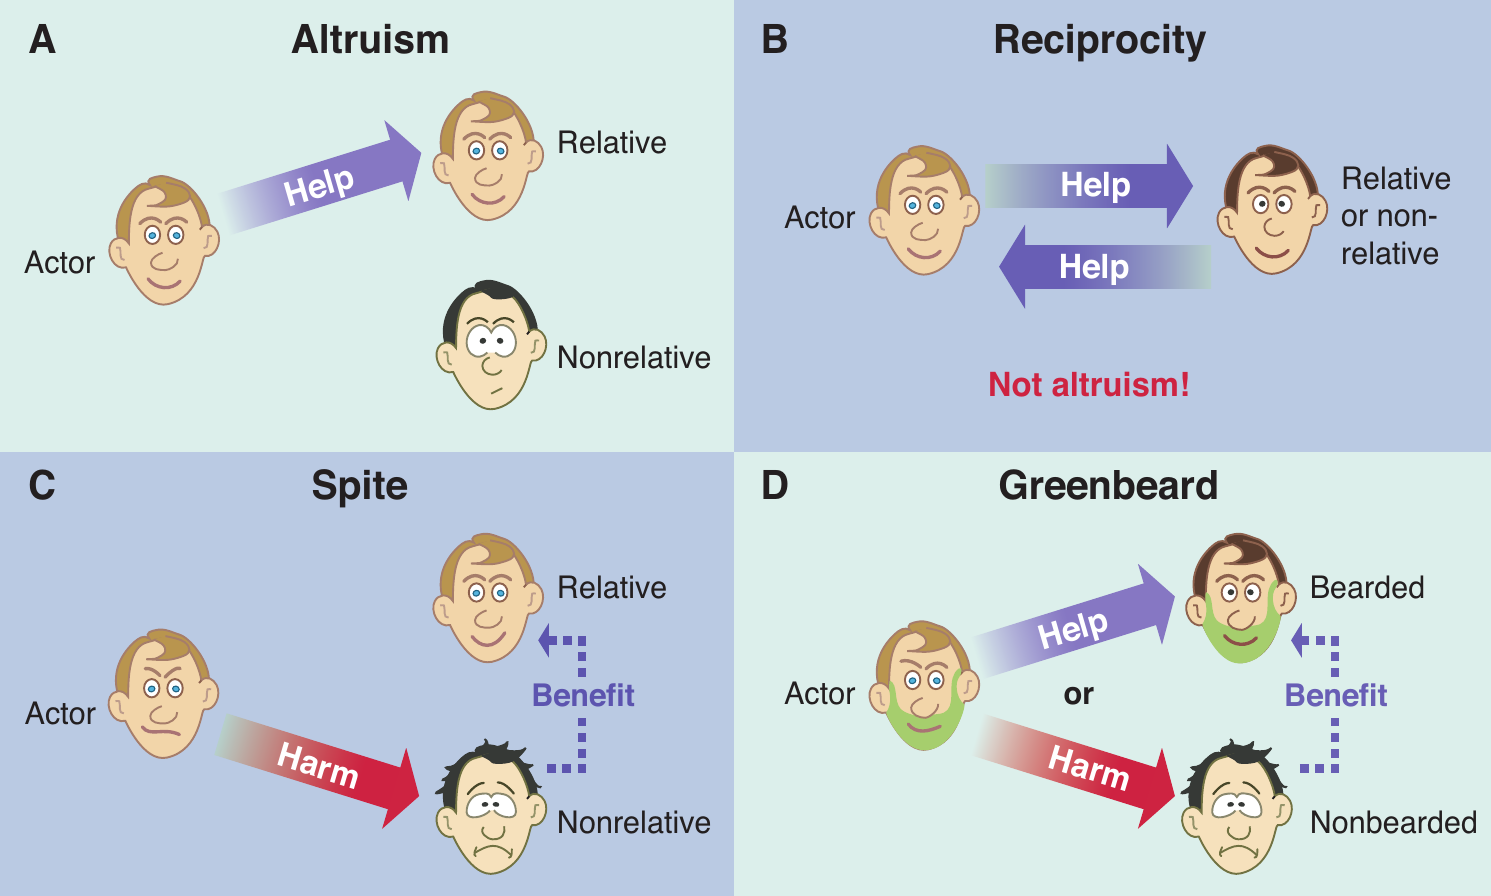
\includegraphics[width=\columnwidth]{figures/mechanisms}
        \caption{Altruism, Reciprocity, Spite, and Green Beard: The four mechanisms describe by \citeauthor{hamilton_kin_1964}'s rule \cite{west_altruism_2010}.}
        \label{fig:mechanisms}
    \end{figure}


    \section{Indirect Reciprocity}\label{sec:indirect_reciprocity}
    Another important concept is the mechanism of indirect reciprocity which is closely related to direct reciprocity (\Cref{reciprocity}) with the difference that reciprocation comes from another individual who is not the original recipient \cite{alexander_biology_1987,boyd_evolution_1989}.
    The significance of this idea stems from the fact that research beliefs that indirect reciprocity played a key role in establishing large-scale human societies \cite{roberts_kin_2019}.
    This importance initially arose when the idea of cooperative reputation, e.g. the image scoring strategy or more sophisticated mechanisms such as the standing strategy \cite{leimar_evolution_2001,ohtsuki_leading_2006}, were proposed that provided an explanation on why indirect reciprocity might work \cite{nowak_evolution_1998}.
    Here, the idea is that donors base their decision of whom to donate to on a score which is based on a recipient's reputation.
    This consequently means that cooperation can occur even if the donor, and the recipient have never met.
    Different experiments conducted in the past support this phenomenon \cite{nowak_five_2006, milinski_cooperation_2002, milinski_reputation_2002,milinski_reputation_2016}.

    A very different view on the idea of indirect reciprocity provides the paper by \citeauthor{roberts_kin_2019} \cite{roberts_kin_2019} where he argues that this type of cooperation is rather driven by relatedness instead of actual reciprocity.

    "[...] individuals do not help other helpers to receive something back from third parties; instead, they help because this features the spread of a strategy of helping those who help others [...]" \cite{roberts_kin_2019}


    Concerning indirect reciprocity via image scoring, \citeauthor{roberts_kin_2019} argues that results from previously conducted experiments have been misinterpreted as evidence for indirect reciprocity.
    For instance, in an experiment by \citeauthor{milinski_reputation_2002} \cite{milinski_reputation_2002}, their result was used to explain indirect reciprocity but it lacked insights whether or not donors actually got higher payoffs by playing the image scoring strategy.
    This is a key problem as higher payoffs are a requirement for indirect reciprocity.
    Furthermore, demonstrating that an individual who plays the image scoring strategy performs better would still not be enough proof for indirect reciprocity via image scoring as self-interested players who want to maximize their own payoff would donate indiscriminately in a population dominated by image scorers as donating more results in higher payoffs \cite{roberts_kin_2019}.
    According to \citeauthor{roberts_kin_2019} the phenomenon which actually needs to be shown is that "those who discriminate most have a higher payoff than those who give to anyone" \cite{roberts_kin_2019}.

    Regarding the idea of image scoring strategies being actually driven by relatedness, \citeauthor{roberts_kin_2019} refers back to \citeauthor{hamilton_kin_1964}'s rule.
    According to \Cref{eq:rb-c} altruism is beneficial if the benefit $b$ for the recipient, scaled by the relatedness $r$ outweighs the costs $c$ of the actor.
    Similarly, \citeauthor{nowak_five_2006} \cite{nowak_five_2006} derive a equation for indirect reciprocity via image scoring:

    \begin{equation}
        qb - c > 0\label{eq:qb-c}
    \end{equation}

    Here, $q$ denotes the social acquaintanceship, i.e. the probability of knowing the recipient's image score.
    Based on this similar notation, \cite{roberts_kin_2019} argues that $q$ is actually relatedness.

    "Individuals should pay the cost of helping when this is offset by the benefit to the recipient multiplied by their chance of sharing the same strategy." \cite{roberts_kin_2019}

    Hence, altruism is selected by means of indirect fitness rather than indirect reciprocity.
    This idea of indirect reciprocity being related to kin selection is summarized in \Cref{fig:indirect_reciprocity}.

    \begin{figure*}
        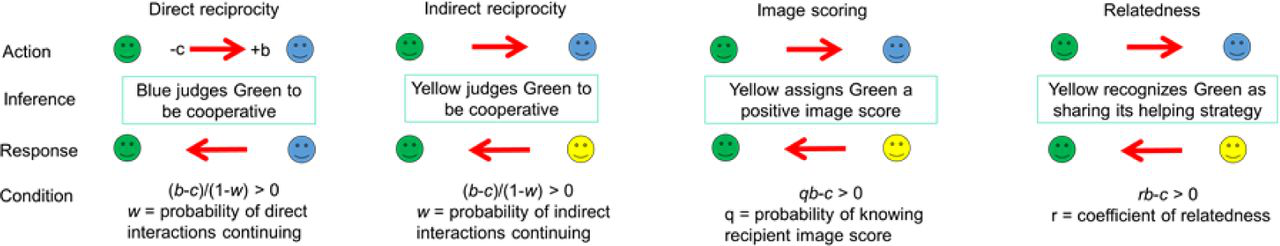
\includegraphics[width=\textwidth]{figures/indirect_reciprocity}
        \caption{The relation/similarity between direct and indirect recprocity, and image scoring and relatedness/the green beard phenomenon \cite{roberts_kin_2019}.}
        \label{fig:indirect_reciprocity}
    \end{figure*}

    \citeauthor{roberts_kin_2019} goes even further and says that reciprocity is an illusion and that the image scores and individual observes are actually cues about kinship.
    Important for our experiments is the idea that in absence of actual relatedness green beard types are observed that help individuals to distinguish between contributors and free riders \cite{roberts_kin_2019}.


    \section{Hypothesis}
    Inspired by the work of \citeauthor{milinski_cooperation_2002} \cite{milinski_cooperation_2002} and the additional insights from \citeauthor{roberts_kin_2019} \cite{roberts_kin_2019}, we found the idea of image scoring and how it can enforce cooperation in a public goods game without/little punishment very interesting.
    Given the idea that this image score is mostly spread via gossip in our society, we pose the question on whether this gossip can always be trusted.
    Similarly to the game "Chinese Whispers/Telephone", we argue that gossip might be altered by some noise over time resulting in a scenario where agents with an actual bad image score might be perceived as being cooperative.
    As a result from that imposters might occur which seem to act cooperatively influencing the overall effectiveness of cooperation.

    Based on this posed question we want explore whether in such a setting cooperation would still outweigh defection or if defection would take over.
    We hypothesise that misinformation or deception has a major influence on the effectiveness of cooperation and that as soon as misinformation gets introduced to the setting altruism via cooperation gets unstable quickly.
    Furthermore, we think that the amount of misinformation does not necessarily play an important role rather if misinformation exists or not.
    Based on the previously mentioned (\Cref{sec:indirect_reciprocity}) relation between indirect reciprocity and relatedness, or image scoring and the green beard phenomenon, we proceed in our experiments with the green beard effect as mean of image scoring mechanism.

    In order to be more concrete, we argue that the more noise is injected in $q$ from \Cref{eq:qb-c} or in other words, the more imposters are prominent, the rarer it is to observe cooperative behaviour.


    \section{Related Work}
    One of the first more extensive studies on information and its influence on a species' fitness was explored by \citeauthor{wallace_misinformation_1973} \cite{wallace_misinformation_1973} where he built upon the claim by \citeauthor{fisherGeneticalTheoryNatural1930} \cite{fisherGeneticalTheoryNatural1930} and proved its correctness, that is, if misinformation is spread it should highly deviate from the truth.
    He explained first why accurate information about one's environment is of great importance and that deception of information results in a loss of the recipient's fitness and formally proved second that slightly misleading information has a probability of one half to improve the fitness of the actor.
    Hence, information must be highly misleading to be truly effective.

    As described in \Cref{sec:indirect_reciprocity}, image scoring is similar to relatedness/the green beard phenomenon which is why the concept of false beards plays a rather significant role for our research.
    Described in multiple papers \cite{SelfishGeneRichard,roberts_kin_2019,west_altruism_2010}, the effect of cheating false beards are directly responsible for the non-existing of cooperative behaviour.
    Here, a false beard describe the act where an entity disguises himself to be a bearer of a green beard allele, but is not.
    Hence, it is purposefully transmitting misinformation regarding is true intentions and, thus taking advantage of the altruism of truthful green beard bearers \cite{SelfishGeneRichard}.
    For this reason, \citeauthor{SelfishGeneRichard} \cite{SelfishGeneRichard} argues that the green beard mechanism is of rare existence, hinting that cooperative behaviour based on the green beard phenomenon is rather unstable if misinformation about true strategy of individuals is spread.

    A more modern and very similar work to ours is the paper published by \citeauthor{szamado_deception_2016} \cite{szamado_deception_2016} where they specifically looked at how gossip mechanisms in indirect reciprocity via image scoring influences cooperation.
    They concentrated on the same idea as we did where they posed the question on how random errors during gossip or even deceptive communication give rise to the collapse of cooperation.
    Therefore, our work is complementary to theirs as we both pursue the same question, however, with a different methodological approach.
    Based on their experiments, they empirically showed that allowing the spread of deceptive information turns the image scoring based reputation worthless and, thus cooperation is rarer or non-existing.
    Additionally, as we expect equal outcomes of our experiments, their findings act as a sanity check for our results.

    In a later work from \citeyear{whitaker_indirect_2018}, \citeauthor{whitaker_indirect_2018} \cite{whitaker_indirect_2018} looked at the evolution of prejudicial groups in indirect reciprocity interactions between actors.
    As prejudice is an opinion about other actors, not based on reason or experience, it is similar to the spread of misinformation concerning the reputation of actors belonging to different groups, hence, explaining the relatedness to our work.
    With the help of computer simulations they were able to show the co-evolution of prejudicial groups and cooperative behaviour, despite the general view of those being opposing forces.
    However, cooperative behaviour is structural limited in a population as prejudice limits cooperation to flourish solely in isolated groups which have the same opinion on outsiders.
    This shows that cooperation can still exist even with perturbed information or intentionally spread lies.


    \section{Method}\label{sec:method}
    This section covers our experiment setup including the different kind of parameters we vary as well as detailed explanations regarding our environment and the logic of the simulations we run.
    In general the situation can be thought of as follows.
    Based on a starting population of \VNumPop, these \VNumPop agents compete for a certain amount of limited resources.
    We cap these at \VNumTrees, but allow one such resource to be shared by two agents, leading to effectively 2 * \VNumTrees resources.
    The reason for this is that two agents sharing a resource can help each other out in the case the resource turns out to be faulty.
    We set \VProbPredator of the resources to be faulty.
    When two agents share such a faulty resource, only one of them randomly gets chosen to live on (if there is only one, it does not live on).
    In the case that an agent is not able to access a resource, it ceases to live.
    This is done over \VNumDays days and averaged throughout \VNumSimulations simulations.
    We simulate this case with a variety of different agent types that act differently and enable various amounts of altruism.
    This manifests itself in the way the non-chosen agent acts when in a faulty resource situation, where e.g. it could choose to share its resource with the agent who obtained a faulty one with the potential to end up dying itself instead.
    We differentiate these by grouping them into four different kinds of tribes/types.

    To give it a more modern spin, we frame the story as being part of the job market.
    Here an agent stands for a contractor, a resource for a job, with a faulty resource corresponding to a difficult job where only one of the contractors gets paid.
    In this simple scenario a contractor goes bankrupt if they cannot find a job for a day \todo{and when simulating the stable population, agents are not able to finish the job on time and both get fired}.
    In altruisitc scenarios, by taking on workload of the hard job from the other contractor who was bound to be fired, one is able to help the other survive with the risk of being fired oneself.

    \todo{Add code step by step, or config for each experiment in the appendix, whole code in general in the appendix}


    \subsubsection*{Experiment 1: Stable Environment}
    To create a general baseline for the simulations to take place in, we implement an environment that on average does not see any large population changes.
    This can be used to compare against in regards to the different types of type/tribe logic when they come across a faulty resource problem.
    Every night the surviving agents reproduce by themselves (asexual, no partner needed) leading to 1 or 2 offspring with a probability of \VProbKids.
    The offspring are of the same tribe as the parent.
    In this baseline case this corresponds to the population only consisting of \cowards which do not help in faulty resource cases.
    These \cowards will be plotted in blue.

    \subsubsection*{Experiment 2: General Altruism}
    For our second experiment we add another tribe to the \cowards, the \suckers.
    We build upon our previous experiment but change the outcome when agents come across a faulty resource.
    These implement altruistic thinking and would always aid the other agent (\suckers and \cowards) that shares the same faulty resource.
    In such a case, the bound-to-die agent gets to live on, while the \sucker now carries the risk of failing.
    If one agents arrives, it simply fails.
    In the case that two agents arrive, one of the two gets randomly chosen to fail.
    We differentiate between the following two cases.
    If the surviving agent is of type \coward, he runs away and lets the other one die.
    If however the survivor is a \sucker, it helps out the to-die one by putting the load from the other agent onto himself.
    With a defined probability of \VProbAltruistDies, the \sucker fails and ends up sacrificing themselves for the other.
    In the other case that it ends up succeeding however, a net-positive is achieved regarding the population as both agents sharing the faulty resource are then able to live on.
    We plot the \suckers in yellow.


    \todo{add code with logic}

    \subsubsection*{Experiment 3: Greenbeard Altruism}
    To introduce a more realistic and fair version of "altruism" we let the \suckers obtain a greenbeard gene which allows them to differentiate between their own kind and \cowards.
    By doing this, in the faulty resource scenario the newly introduced \greenbeards decide to only help out other \greenbeards that would return the favour if the positions were changed.
    Thus in the third experiment, we analyze how the population fares when it consists of 50\% \cowards and 50\% \greenbeards.
    This should ensure that the population of the \altruists are able to hold together and increase in size while the number of non-cooperative \cowards gets reduced.

    \subsubsection*{Experiment 4: On Trust and More}
    \todo{A final experiment introduces further types next to the altruist.
    The final types are \cowards (never help with hard jobs), \suckers (always help with hard jobs), \impostors (look like altruists, but never help) and  \greenbeards (only help other altruists, aka \impostors and \greenbeards).}


%    {
%        This section should describe the method of your \emph{final} submission in detail. This includes things you did with the data (e.g. preprocessing, augmentations, changes of representation, etc.) and the actual definition of your model. Sometimes it is fine to describe a model in text or math only, sometimes it is better to create an overview figure. Either way, after reading this section, a reader should be able to implement your architecture.
%        If you have enough space, you may list hyperparameter values in an ``Implementation Details'' paragraph. Otherwise list them in the README of your code repo.
%    }
%
    \todo{
        Algorithms regarding matching
        \cite{geffen_efficient_2017}
        average birth and death rate per day. this would illustrate why convergence is rather slow}


    \section{Results}\label{sec:results}
    In the following section we present the results of our experiments.

    We note that for our hypothesis and insights we primarily look at the average of the results of our \VNumSimulations simulations.
    The colours denote the different kinds of tribes/types and their respective behaviours when they are the survivor in a faulty resource situation.
    Blue stands for \cowards which never help out.
    Yellow denotes \suckers which always help out.
    Red stands for \impostors which appear to others as they would help out but in fact do not.
    Green denotes \greenbeards which help out other seemingly altruistic agents (aka suckers, greenbeards and impostors).

    \subsubsection*{Experiment 1: Stable Environment}
    As our first step, we create an environment so that our population neither goes extinct, nor explodes in size within the \VNumDays days timeframe we have set.
    \todo{This acts as a comparison for the quality of further experiments.}
    As can be seen in \Cref{fig:stable_pop} while there notably is one large deviation, averaging over \VNumSimulations runs the starting population of 100 stays roughly the same.

    \begin{figure}
        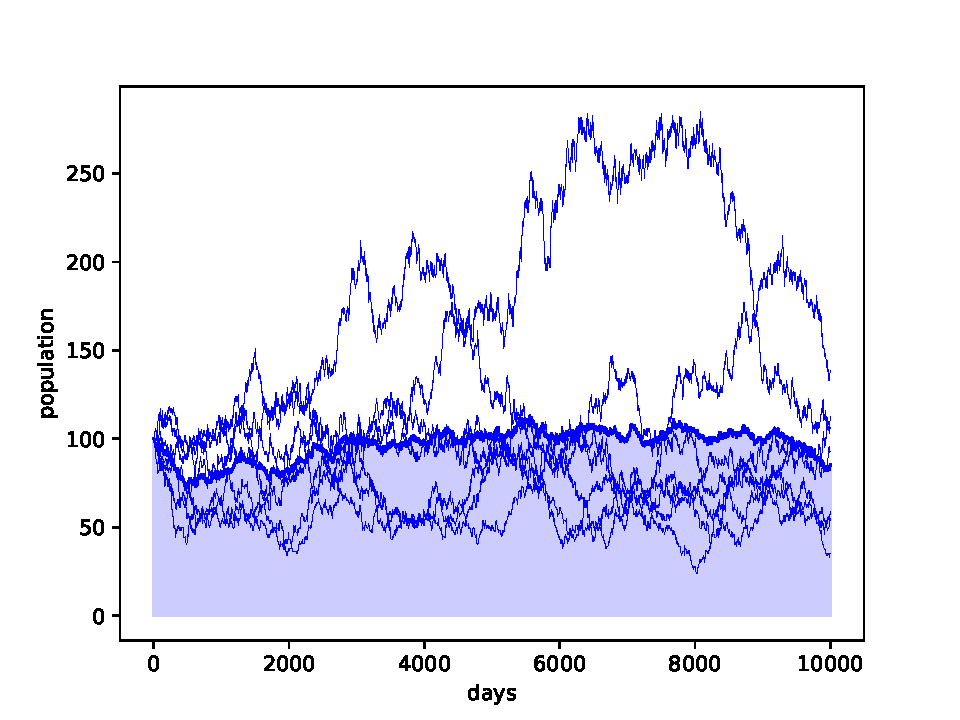
\includegraphics[width=\columnwidth]{figures/exp1_stable_pop}
        \caption{\textit{Exp 1:} Without any sort of tribe logic, the populations consists of solely \cowards.
        With some deviations, the population stays on average roughly the same at around \VNumPop.
        Visualized are \VNumSimulations random runs in light and their average in dark blue. }
        \label{fig:stable_pop}
    \end{figure}


    \subsubsection*{Experiment 2: General Altruism}

    We now analyze a more sophisticated way of survival by introducing concepts of collaboration and altruism.

    A first run shows that, as expected, introducing altruistic thinking leads to an increase in population size, visualized in \Cref{fig:alt_cow_total}.
    The population also reaches saturation pretty early on around day 1.500.

    \begin{figure}
        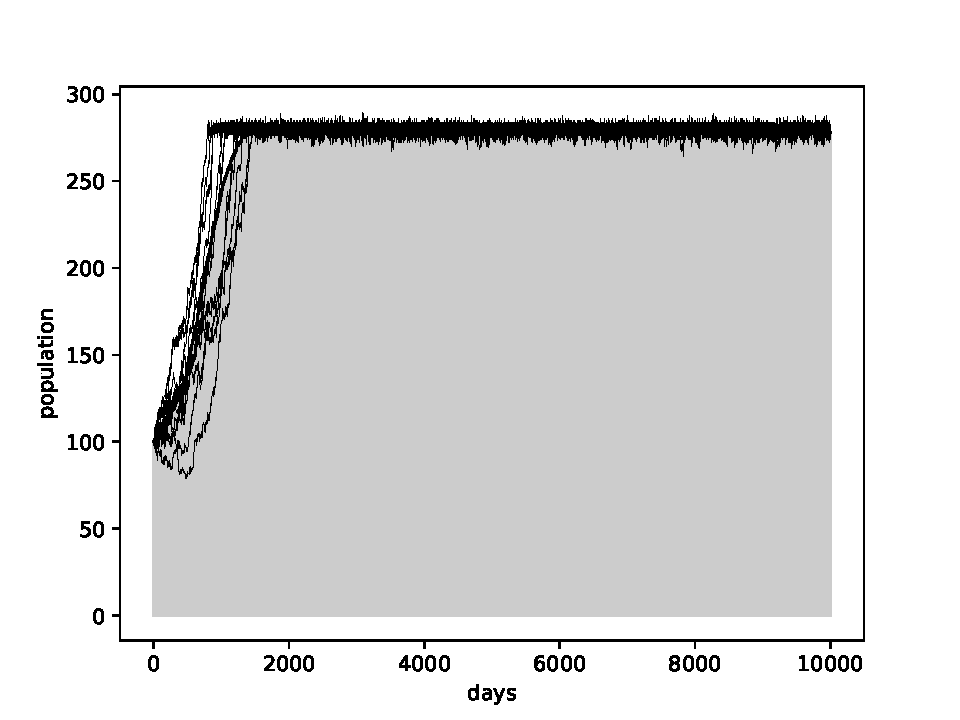
\includegraphics[width=\columnwidth]{figures/exp2_total}
        \caption{\textit{Exp 2:}As compared to the baseline case, introducing altruistic thinking leads to a big increase in and early saturation of population size.
        }
        \label{fig:alt_cow_total}
    \end{figure}

    We further analyze how this effect gets spread between the two types of agents.
    In \Cref{fig:alt_cow_separated} we see that the amount of \suckers (aka altruists that help everyone) decreases steadily, while the population in general increases.
    This figure also shows that the amount of \cowards substantially increases.
    A potential explanation for this could be that in general the birth-rate for the \altruists is much lower than their die-off rate given their altruistic sacrifices.
    The cowards on the other hand, while having the same birth-rate, experience lower die-off-rates due to running away from a predator instead of helping.
    If we compare this to the original experiment without any altruism (\Cref{fig:stable_pop}), we see that this altruistic thinking has a large net-positive effect.
    This is the case even though the \suckers do not differentiate between whom they save.
%    \todo{play around with settings so that they do die out and the following experiment makes more sense}

    \begin{figure}
        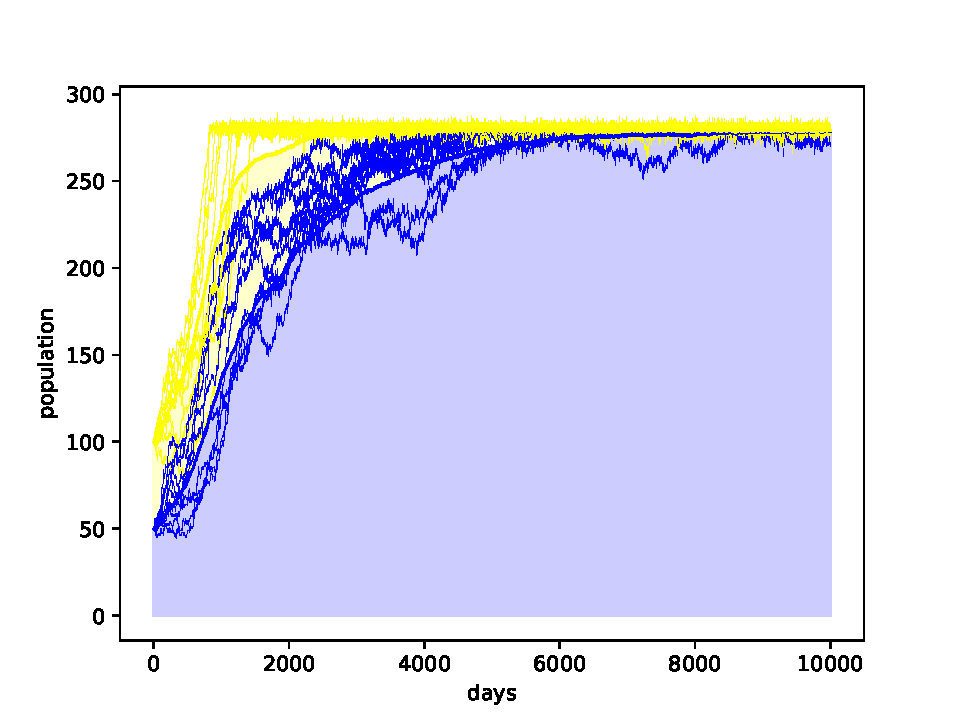
\includegraphics[width=\columnwidth]{figures/exp2_sucker}
        \caption{\textit{Exp 2:} Altruistic thinking leads to a large absolute increase in population.
        A saturation occurs around day 1.000, after which the increase in \cowards starts to slow down a little.
        By day 5.000 there are virtually no \suckers.}
        \label{fig:alt_cow_separated}
    \end{figure}

    In the following \Cref{fig:alt_cow_separated_rel} we see how these different types stack against each other when compared in relative terms.
    With a sharp increase right at the beginning on, $\sim 80\%$ of the population consists of cowards by day 2500.
    While there are some runs where the \suckers were able to gain traction and constitute close to the majority at around day 1.000, by day 5.000 the population consists of 99\% \cowards with the \suckers going extinct in most runs.


    \begin{figure}
        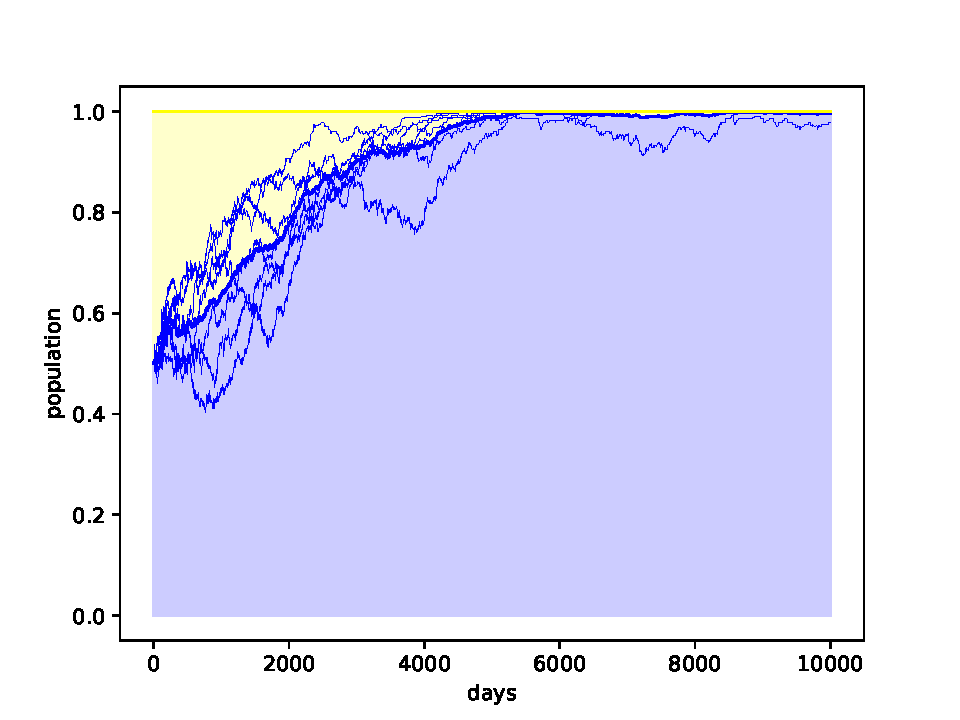
\includegraphics[width=\columnwidth]{figures/exp2_sucker_rel}
        \caption{\textit{Exp 2:}With altruistic thinking the proportion of \suckers declines linearly, reaching 0 after around 5.000 days on average.}
        \label{fig:alt_cow_separated_rel}
    \end{figure}



    \subsubsection*{Experiment 3: Greenbeard Altruism}
    In the previous experiments we have seen that the \cowards experience an increase in population, while the \suckers/\altruists themselves do not benefit all too much (besides the net increase in general population).
    To fix this unfairness/inequality and introduce another experiment we consider the case where \altruists (here now \greenbeards) only help each other out.

    Looking at \Cref{fig:exp3_greenbeard} we can see that our previously mentioned hypothesis is the case.
    The amount of \greenbeards increases substantially, while the number of \cowards drops equivalently, seemingly converging towards zero.
    We see that there is a general positive trend to be made out.
    This can further be seen in \Cref{fig:exp3_greenbeard_rel} where we have plotted the relative distribution of the different types.
    Interestingly enough, within the first 1.000 days, the number of \cowards seems to improve faster in relative and absolute terms.
    As soon as the population starts to saturate, the composition of the population shifts, with the proportion of \cowards reducing linearly.
    At day 2.000 the \greenbeards take up 50\% of the population, reaching 80\% at day 6.000 and 90\% by the end of day 10.000.



    \begin{figure}
        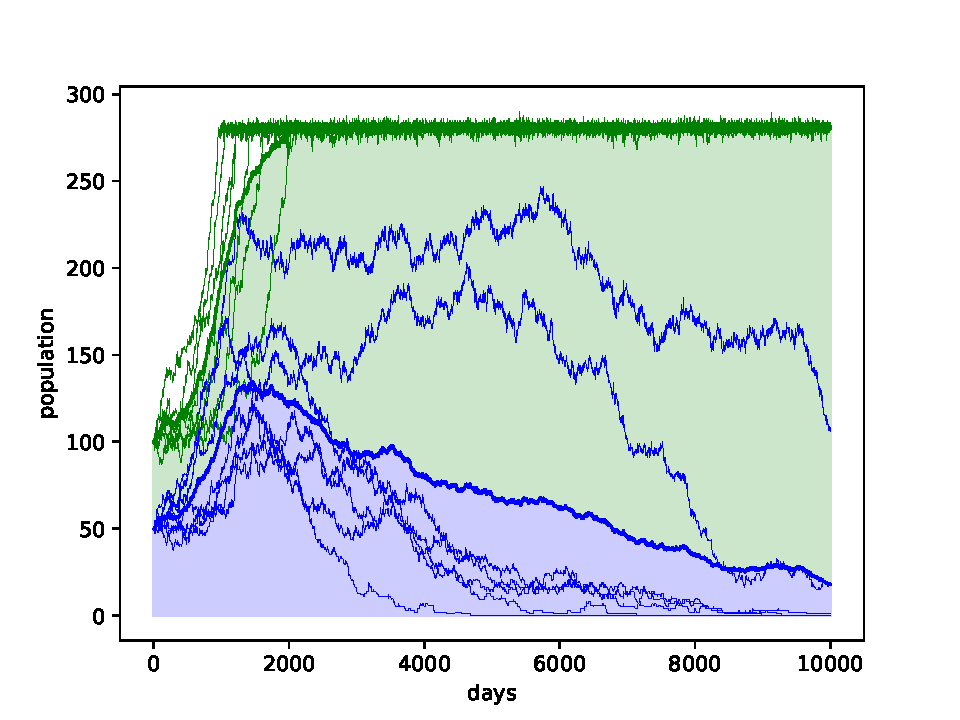
\includegraphics[width=\columnwidth]{figures/exp3_greebeard}
        \caption{When introducing \greenbeards that only help each other out, we see an increase in \cowards up until day 2.000 when the population saturates.
        After that the \greenbeards take over substantially.}
        \label{fig:exp3_greenbeard}
    \end{figure}


    \begin{figure}
        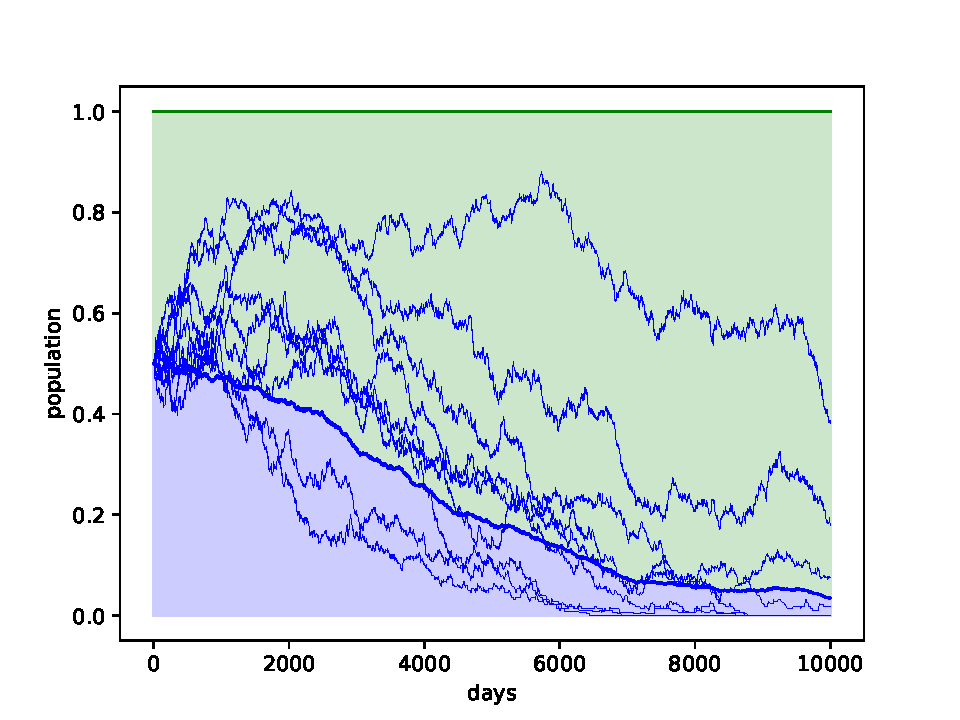
\includegraphics[width=\columnwidth]{figures/exp3_greenbeard_rel}
        \caption{From a relative standpoint we see that the \greenbeard gene leads to a change in population composition.
        Constituting 42\% of the population at day 1.000 the \greenbeards end up at over 90\% by day 10.000.}
        \label{fig:exp3_greenbeard_rel}
    \end{figure}

    \subsubsection*{Experiment 4: On Trust and More}
    \todo{
        In the evaluation section you should describe the experiments that support the claims of the story of your report. For example, if you previously said ``We propose to combine model A with component B which leads to improved accuracy.'' you should back this up with experimental evidence here. Typically, this means that you should show the performance of model A with and without component B. May be your method warrants other kinds of such ablation studies, which you might include and describe here.

    }


    \section{Discussion}\label{sec:discussion}
    \todo{
        Sometimes you might have had a great idea, but it did not pan out. Since we want to encourage novelty, such failed attempts should also go into the report. This section is a suitable place to discuss this. If you can, do not just list failed attempts, but actually \emph{discuss} them, i.e., provide an intuition why you think they failed or what the problem is that prevented them from performing better. It is much better to describe one failed attempt and discuss it in-depth than just listing four failed models without any explanation.

        If you do not have failed attempts that would warrant their own section, this is perfectly fine. You may discuss the experiments from the previous section here, or if you prefer to have the discussion the evaluation section directly, feel free to omit this section entirely.

    }


    \section{Conclusion}\label{sec:conclusion}
    \todo{
        Conclude your report with a brief summary. This can be very short, i.e. 2-3 sentences.
    }
    Lastly, they mention how countermeasures, i.e. employing punishment, which maintain a truthful image scoring system allow cooperation to be restored again. \cite{szamado_deception_2016}
    \bibliographystyle{ACM-Reference-Format}
    \bibliography{bibliography}

\end{document}
